
\documentclass[en]{ujdpl}

\usepackage[polish]{babel}
\usepackage[utf8]{inputenc}
\usepackage{ae}

\usepackage[T1]{fontenc}

\usepackage[justification=centering]{caption}

\usepackage{url}
\usepackage{latexsym}
\usepackage{textcomp}

\usepackage{titlesec}
\usepackage{graphics} % wlaczanie grafik
\usepackage{wrapfig}

\usepackage{color} % kolory
\usepackage{floatflt}
\usepackage{bookmark}
\frenchspacing
\usepackage{indentfirst}

% dodatkowe pakiety
\usepackage{amsmath}
\usepackage{multirow}
\usepackage{enumerate}
\usepackage{listings}
\usepackage[usenames,dvipsnames]{xcolor}
\lstloadlanguages{xml}

\hyphenpenalty=100000

\definecolor{listinggray}{gray}{0.9}
\definecolor{lbcolor}{rgb}{0.9,0.9,0.9}
\lstset{
	backgroundcolor=\color{lbcolor},
	tabsize=4,
	rulecolor=,
	language=xml,
        basicstyle=\scriptsize,
        upquote=true,
        aboveskip={1.5\baselineskip},
        columns=fixed,
        showstringspaces=false,
        extendedchars=true,
        breaklines=true,
        prebreak = \raisebox{0ex}[0ex][0ex]{\ensuremath{\hookleftarrow}},
        frame=single,
        showtabs=false,
        showspaces=false,
        showstringspaces=false,
        identifierstyle=\ttfamily,
        keywordstyle=\color[rgb]{0,0,1},
        commentstyle=\color[rgb]{0.133,0.545,0.133},
        stringstyle=\color[rgb]{0.627,0.126,0.941},
}


\lstdefinelanguage{JavaScript}{
  keywords={typeof, new, true, false, catch, function, return, null, catch, switch, var, if, in, while, do, else, case, break, this},
  keywordstyle=\color{blue}\bfseries,
  ndkeywords={class, export, boolean, throw, implements, import},
  ndkeywordstyle=\color{}\bfseries,
  identifierstyle=\color{black},
  sensitive=false,
  comment=[l]{//},
  morecomment=[s]{/*}{*/},
  commentstyle=\color{purple}\ttfamily,
  stringstyle=\color{red}\ttfamily,
  morestring=[b]',
  morestring=[b]"
}

\lstset{
   language=JavaScript,
   backgroundcolor=\color{listinggray},
   extendedchars=true,
   basicstyle=\footnotesize\ttfamily,
   showstringspaces=false,
   showspaces=false,
   numbers=left,
   numberstyle=\footnotesize,
   numbersep=9pt,
   tabsize=2,
   breaklines=true,
   showtabs=false,
   captionpos=b
}


% paragraph gap:
\setlength{\parskip}{0.5\baselineskip plus 0.5ex minus 0.2ex}

%---------------------------------------------------------------------------

\author{Sebastian Poręba}
\shortauthor{Sebastian Poręba}

\title{Comparison of 3D physics engines}

\shorttitle{Comparison of 3D physics engines}

\thesistype{Praca magisterska}

\supervisor{dr hab. Paweł Węgrzyn}
\consultant{mgr Bartosz Porębski}

\date{2013}

\faculty{Wydział Fizyki, Astronomii i Informatyki Stosowanej}

\acknowledgements{I would like to thank my advisors Paweł Węgrzyn and Bartek Porębski. Also I need to thank Collin Hover and Ibon Tolosana for their valuable insights and help with tests.}

%---------------------------------------------------------------------------

\begin{document}

\titlepages

\setcounter{tocdepth}{1}
\tableofcontents

\clearpage

\newcommand{\sectionbreak}{\clearpage}

\chapter{Introduction}
\label{cha:introduction}

The main objective of the presented project is the implementation of parts of 3D engine in a browser environment. Parts of the engine are analysed side-by-side with a parallel engine compiled from C++. The objective of the analysis is to compare performance and describe possible issues related to the limited browser resources and dynamic features of JavaScript.

At the moment of writing, the majority of games are developed with C++ and usually DirectX. These technologies are mature and have excellent performance. Features of the language give flexibility and high-level solutions to effectively manage application (e.g. operator overloading, multiple inheritance) and enable to fine-tune the internals of application to achieve best execution times. For games with high budget\cite{gta} C++ is an obvious choice for having the best possible result.

However, in parallel to the AAA game industry, the casual and independent games sector is growing. In 2013, the market is expected to be worth \$8.64 billions in total. A total of 2.4 billion tablets and smartphones with casual games capabilities will be reached before the end of 2013. These games are less focused on creating cutting edge graphics and physics simulations and more on overall experience and social interactions.

JavaScript is a scripting language not designed to perform high-load computations. However, at present it is the only language widely supported by all browsers. With all it's advantages and quirks is the only choice available for programmers.\footnote{Currently two new languages are being developed -- Dart by Google and TypeScript by MicroSoft. However, to enable cross-compilation to JavaScript, the paradigm of these languages is similar and work is focused mainly on better IDE support.}

While suffering from design issues, JavaScript provides a complete environment that makes development very easy for both beginner and advanced programmers. Two very important components of every application are provided out of the box -- a rendering system and networking in the browser. They were designed for HTML pages to carry mainly text information, they are still suitable for gaming. Building a simple 2D game is often a matter of few hundred lines of code responsible for transferring user input to the positions of sprites defined in CSS. This is clearly visible during competitions like JS13kGames\cite{js13kgames} where all game assets and the code have to be fitted into 13kB package.

Many projects varying from server side solutions\cite{nodejs,coder} to hardware developer boards\cite{espruino} are taking advantage of this simplicity. From the perspective of game development, it is unlikely at the time of writing that an AAA game may be created to run in the browser. However, growing segments of casual, independent and social games are already targeting the web as a platform.

\section{Influence on the distribution process}

Traditionally, games are often still sold in actual boxes and some update system is always incorporated to patch any bugs appearing after initial release. Systems like Steam\cite{steam} are making this process easier, but still suffer from the necessity of having to install a game on the hard drive.

Creating an application that works in the browser simplifies distribution significantly. All assets and code are downloaded each time the user enters a website, so no update system is necessary -- all users are always playing the latest version. Usually browser games are monetised differently to traditional titles. Playing a basic version is usually free and earnings come from either ads or premium content. This is completely new approach, present also in MMO\footnote{Massive Multiplayer Online} games. It resulted in psychological research on leveraging compulsive behaviours to maximise profits\cite{exploitative-game-design}.

Working in a browser gives access to all social networks of users, so usage of Twitter or Facebook based features is very simple -- which boosts the promotion of the game. It also enables, though morally questionable, to target people who are not able to install games on company issued computers. Disallowing games in browsers is a far more complicated task for administrator, similar to blocking ads or mature content.

Lastly, the web is better suited to run easily on all platforms. The browser is a layer of abstraction that is transparent for the application, whether it runs on any traditional operating system, gaming console or mobile device. Of course performance and screen size should be taken into consideration, but ability to write one codebase that runs on multiple devices has already encouraged projects that package JavaScript applications as native ones\cite{phonegap}, greatly reducing development costs for the growing variety of phones and tablets.

\begin{figure}[h!]
  \caption{Game created with ImpactJS}
  \label{img:impactjs}
  \centering
	\includegraphics[width=12cm]{summary/impactjs.png}
\end{figure}

Multiple open-source and commercial game engines are being created lately. Examples worth mentioning are ImpactJS\cite{impactjs}, Turbulenz\cite{turbulenz} and Isogenic Engine\cite{isogenicengine}.


\begin{figure}[h!]
  \caption{Game created with Isogenic Engine}
  \label{img:isogenic}
  \centering
	\includegraphics[width=12cm]{summary/isogenic.png}
\end{figure}

A very important and growing sector is interactive 3D arts with two major targets -- music videos and commercials. They are uniquely available only in browsers as a very viral extensions of regular marketing. One of the first occurrences of this technology was the video for Rome music group: "3 dreams of black"\cite{rome}. The project allows to move the camera while an animated 3D story is rendered alongside the music. After the movie is over, the user is allowed to create 3D models that are later incorporated into the experiences of other people watching. This way interactions and social element are enabled in what used to be a one-way transmission of art form.

\begin{figure}[h!]
  \caption{Screenshot from "3 dreams of black"}
  \label{img:rome}
  \centering
	\includegraphics[width=12cm]{summary/rome.jpg}
\end{figure}

\section{Technology}

The browser-based engine is implemented in JavaScript and analyzed in V8 engine. V8 is maintained by Google and is used in the Google Chrome browser. Executable examples are compiled using gcc compiler and are run on the same platform. For additional comparison, the Emscripten project is used to automatically generate JavaScript and measure if the automated conversion may be as effective as writing code by hand.

The project is based on conference sessions and announcements authored by V8 programmers regarding the performance of JavaScript applications. The analysis of available materials is a topic of Chapter 2, where internals of modern engines for dynamic languages are briefly explained.

Chapter 3 covers particles often used to simulate loosely connected systems like smoke, fire, fog, etc. It shows techniques of memory allocation and garbage collection that help improve performance. Two particle systems are presented -- one with high memory allocation that is expected to cause performance issues and the second one, improved by the usage of object pools.

Chapter 4 focuses on sphere collision detection and reaction, with both naive solution and space partitioning using Octree. This benchmark shows an application with high CPU usage and relatively simple math computations. Because of this simplicity, collision detection with spheres is almost always used as a preliminary method of eliminating collision between objects. More complex and expensive algorithms are used to determine the real state of such a pair only if bounding spheres are colliding.

The systems presented in chapters 3 and 4 are not targeted to be full physics engines. They are however representative to general concepts encountered in every game.

Chapter 5 describes Emscripten, a project aimed to convert complete C++ projects to JavaScript. A related library, asm.js, is presented with an overview of architectural choices, which lead to better performance. The generated code is compared to the one created in previous chapters.

The last chapter is a summary of all achieved results. The limitations of JavaScript engines are presented alongside future possibilities for the gaming industry.

Benchmarks are by no means a complete physics system and do not represent the current state of the art of physics algorithms. They are aimed to resemble optimal algorithms in used methods and complexity, so that benchmarks reflect how an actual engine uses memory and computing power.


\chapter{Overview of JavaScript and V8 engine architecture}
\label{cha:overview}

Historically, JavaScript was considered an untyped language, meaning that values had no types attached to variables, either by the programmer or the compiler. All variables were of a single, unified type, and procedures called unboxing and boxing, performed before and after each operation on a variable, ensured that it was properly used on the machine code level. The complete code source was sent from the server to the browser and was parsed and executed on the fly. Without types attached to variables, all functions were polymorphic and unstable, since parameters may have carried any type of variable. To solve this problem, the source code of the function was parsed every time it was called, each time generating a machine code based on current parameters and variables in scope. This approach, called interpretation, is still present in JavaScript engines, and used whenever variables do not match set criteria of stability described later in this chapter.

This paper uses as an engine of choice V8 Crankshaft. This choice was made, because it is the only engine available at the moment which provides direct command line access, enabling the precise performance measurements of code parsing and execution, without browser context and overhead. The executable file of V8 (named d8) is compiled with consideration to the target platform.

\section{JIT compilation -- tracking variable types}
\label{sec:JIT}

As it was mentioned before, initially JavaScript was treated as an untyped language. With the release of SpiderMonkey in Firefox 3.5 in 2009, the situation changed. The first Just-In-Time compiler for JavaScript, TraceMonkey, was created. Based on the works of Prof. Dr. Michael Franz on TraceTrees \cite{Franz94code-generationon-the-fly:} JIT compiler collected all paths that the interpreter took with specific types of variables. A path could split into different methods or if statements. Whenever part of the code was executed often enough, the path was marked as hot, and the compiler optimised it for given types. If a single path was traversed with a different set of types, the compiler could generate another version of the optimised code. When the path turned out to be highly polymorphic, optimised versions were removed and the interpreter was used as a fallback.
Initial reports show speedups between 20x to 40x \cite{firefox-to-get-massive-javascript-performance-boost}.
However, trace JIT turned out to be very complicated to maintain \cite{improving-javascript-performance-with-jagermonkey} and eventually was removed from Firefox in 2011.\cite{trace-jit-removed-from-firefox}. At the time SpiderMonkey was already equipped with JagerMonkey, JIT engine based on method calls. Instead of collecting complete traces, only method calls are counted. This provides easy tracking of function parameters and variables in scope.

\begin{figure}[h!]
  \caption{JIT compiler tracking method calls}
  \label{img:jit-1}
  \centering
	\includegraphics[width=8cm]{jit-1}
\end{figure}


\begin{figure}[h!]
  \caption{JIT compiler marking one of methods as hot and recompiling}
  \label{img:jit-2}
  \centering
	\includegraphics[width=8cm]{jit-2}
\end{figure}

This proved to be more effective and a simpler approach, which is now used in all JavaScript engines. In V8 Crankshaft, a step forward was taken, and simple methods are compiled even before any statistics on data types are collected. For compiled methods the source code is not stored. Instead, a procedure called deoptimisation is implemented. Whenever an engine detects that a compiled code does not match actual types of variables, the code is deoptimised and either optimised again to match the new, better set of variables, or kept in interpreter-friendly form.

To track these changes two debug options for V8 are available: --trace-opt and --trace-deopt.

\lstinputlisting[caption=Output from V8 debug run showing optimisation and deoptimisation,label=listing:optdeopt]{optdeopt.txt}


\section{Type inference}
\label{sec:typeference}

V8's method of optimising code before it is run relies on type inference. Based on the context of the variable its type is guessed. The generated assembler has to support cache miss -- whenever inferred type turns out to be incorrect, a new type is assigned and another JIT compilation runs. Types of variables are organised in a tree, where the Number object may store both Float or Integer, Integer may store SMI (small int), etc.

\lstinputlisting[caption=Tree of types in JavaScript,label=listing:typestree]{types.txt}

In V8 type inference is tightly connected with JIT compilation and may be tracked with the same flags: --trace-opt and --trace-deopt. 

\section{Hidden classes}
\label{sec:hiddenclasses}

JavaScript is a classless language. Object may have defined a prototype which behaves similar to base class in other langauges. However, a property may be added to an Object or its prototype at any point in runtime. To optimise such a dynamic representation, engines use the concept of hidden class. Whenever an Object is created, its hidden class is pointed to the base, empty Object representation. Then each definition of new property makes a transition on the hidden class graph, introducing hidden classes that are not yet defined, as in the following example:

\begin{figure}[h!]
  \caption{Initial shape of hidden class for Point}
  \label{img:point0}
  \centering
	\includegraphics[width=8cm]{point0}
\end{figure}
\begin{figure}[h!]
  \caption{Shape of hidden class for Point after x property added}
  \label{img:point1}
  \centering
	\includegraphics[width=8cm]{point1}
\end{figure}
\begin{figure}[h!]
  \caption{Shape of hidden class for Point after y property added}
  \label{img:point2}
  \centering
	\includegraphics[width=8cm]{point2}
\end{figure}

Based on hidden class the JIT compiler optimises methods to generate an even simpler assembly code similar to the one compiled from C++. Class shape defines address offsets of Object properties. Thus, the hidden class graph is actually a tree, where one class cannot be reached in more than one way.

\begin{figure}[h!]
  \caption{Two point representations based on order of declared properties}
  \label{img:point_tree2}
  \centering
	\includegraphics[width=8cm]{point_tree2}
\end{figure} 

At the moment of writing, the type of property is not tracked in hidden classes. The only exception are primitive values (see Listing \ref{listing:typestree}). In other words, storing an object in property results in the same hidden class, regardless of the hidden class of this object.

Transitions between hidden classes can be tracked in V8 using flags --trace-generalization tracking when variables are cast to a more generic type (e.g. SMI to Integer, or Integer to Number) and --trace-migration (tracking when hidden classes are migrated).

\lstinputlisting[caption=Log of migration trace in V8,label=listing:migration]{migration.txt}

\section{Garbage collection}
\label{sec:garbagecollection}

Memory in JavaScript is managed automatically. Each allocation places an object on a memory heap. The first generation of garbage collection traversed the whole tree and freed memory for all inaccessible objects. This type of deallocation is called mark-sweep and takes a long time. Since JavaScript is single-threaded, this operation blocks all other operations. To improve performance, especially in games, the incremental scavange method of garbage collection was introduced. The engine tracks the age of objects, allowing to quickly detect objects allocated temporarily (e.g. for a single frame rendered in a game). When the object is inaccessible, it is queued for deallocation, in chunks that do not cause long UI freezes.\cite{cheneys-algorithm,garbage-collection}

\lstinputlisting[caption=Log of garbage collection in V8,label=listing:gc]{gc.txt}

\chapter{Particle system}
\label{cha:particlesystem}

Particle system is one of most commonly used techniques to simulate smoke, fire, rain and other groups of discrete objects, usually independent from each other. The system consists of a defined number of emitters, producing lightweight particle objects with certain parameters. Each emitter has a defined production ratio, and each particle a certain lifespan, resulting in the upper limit of total particles on the screen. Some systems also use attraction points, which enable better control over particles, using equations often similar to those of electrostatic forces.
Such simulation is independent from rendering. The same particle system can be used for different effects with proper configuration.

\begin{figure}[h!]
  \caption{Example rendering of tested particle system}
  \label{img:particles}
  \centering
	\includegraphics[width=16cm]{particles}
\end{figure}

\section{System parameters}
\label{sec:emittersparameters}

The tested system works on the two-dimensional Cartesian plane. For the purpose of performance analysis, movements are calculated based only on frames rather than actual flow of time. This means that systems with a different framerate will result in different visualisations, but requesting a given amount of frames rendered will result in the same lifespan and total number of particles in both systems.

Emitter supports the following parameters:

\begin{itemize}
	\item position -- initial position of created particles
	\item angle -- angle counting clockwise from the vector [0, 1]
	\item spread -- parameter controlling random differences in the initial angle of particles
	\item velocity -- initial velocity of particles, in pixels per frame
	\item velocity spread -- parameter controlling random differences in the initial velocity of particles
	\item lifespan -- initial lifespan of particles
	\item productionRate -- amount of particles initialized in each frame
\end{itemize}

A Particle has similar properties:
\begin{itemize}
	\item position
	\item velocity
	\item lifespan
	\item age -- counted in frames, when for given particle it is higher than its lifespan, particle is removed from the system
\end{itemize}

Source code of both implementations is attached in the Appendix \ref{cha:sourcecode}.

\section{Implementation with high memory allocation}
\label{sec:particlesinitial}

The initially tested implementation has one very important property of a particle emitter. Whenever new particles are created, a new array of pointers is allocated and returned from the emitter. The system appends new particles to the existing array. In each frame, the particle system creates a new, empty array of particles and adds only particles that are still alive. The array from the previous frame and all dead particles are removed from the system and deallocated. This is clearly a suboptimal solution that allocates and deallocates plenty of memory in each frame. The purpose of this exercise is to show how both languages handle a bad code, and how big impact it has compared to the optimal solution.

\lstinputlisting[caption=Time measurement of unoptimized particle system in JavaScript,label=listing:timejs1]{particles/timejs1.txt}
\lstinputlisting[caption=Time measurement of unoptimized particle system in C++,label=listing:timecpp1]{particles/timecpp1.txt}

Time measurement shows that the JavaScript version is almost 8 times slower than the native one. To analyse the situation --prof and --log-timer-events flags may be used. The output file v8.log is parsed using an available online tool.\cite{v8-profile-plotter}

\lstinputlisting[caption=Profiler output for unoptimized particles,label=listing:particles1profile]{particles/particles1-profile.txt}

Methods prefixed with ~ are unoptimized, the ones prefixed with * are JIT compiled. As seen in the profiler log, most of the time is spent in unoptimised versions of verifyIfAlive and stepParticle methods.

\lstinputlisting[caption=Annotated part of source,label=listing:particles1stepannotated,language=JavaScript]{particles/particleSystemstep.js}

The same methods are also used in optimised versions, where they take significantly less ticks to run. It is clear that the presented code not only allocates and deallocates too much memory, but also fails to run in optimised mode. It is visible on the chart obtained from the same tool -- stripe labelled "code kind in execution" shows multiple kinds of code running and is interrupted often with garbage collection cycles.

\begin{figure}[h!]
  \caption{Chart of time used in unoptimised verion of JavaScript}
  \label{img:particles1profile}
  \centering
	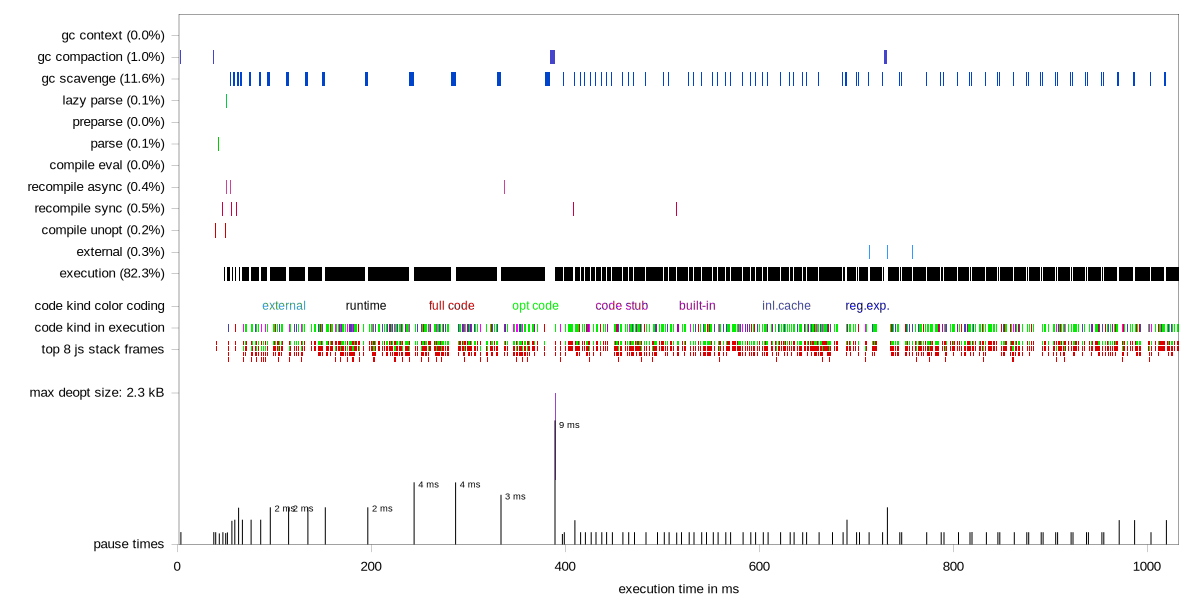
\includegraphics[width=16cm]{particles/particles1-profile.png}
\end{figure}

Garbage collection cycles blocking execution are also visible with --trace-gc flag.

\lstinputlisting[caption=Garbage collection in unoptimised particle system,label=listing:particles1gc]{particles/particles1gc.txt}

\section{Implementation with object pool}
\label{sec:particlesobjectpool}

To improve performance, a different approach to particles allocation is used. Each particle has a flag "isDead" telling if it may be safely reused for a new particle. The particle pool is kept along with a list of pointers to dead particles. This way, when the system reaches its maximum congestion (around 15000 particles in the given example) no new allocations occur.
The creation of new particles is moved from the particle emitter to the particle system, to avoid allocation of the new array. The emitter works now as a structure describing behaviour, but not implementing one.

\lstinputlisting[caption=Time measurement of optimized particle system in JavaScript,label=listing:timejs2]{particles/timejs2.txt}
\lstinputlisting[caption=Time measurement of optimized particle system in C++,label=listing:timecpp2]{particles/timecpp2.txt}

The optimised version shows overall improvement of 85\% for JavaScript and 45\% for C++ making the JavaScript version only 2.2 times slower than the native one. It is clearly visible that JavaScript is more sensitive to unwise memory management.

\lstinputlisting[caption=Profiler output for optimized particles,label=listing:particles1profile]{particles/particles2-profile.txt}

Profiling shows that the step method of the particle system is now always running in optimised mode, and almost no time is spent on other methods. The same is visible on the profiling chart, where the "code kind in execution" stripe shows only the optimised code.

\begin{figure}[h!]
  \caption{Chart of time used in optimised verion of JavaScript}
  \label{img:particles2profile}
  \centering
	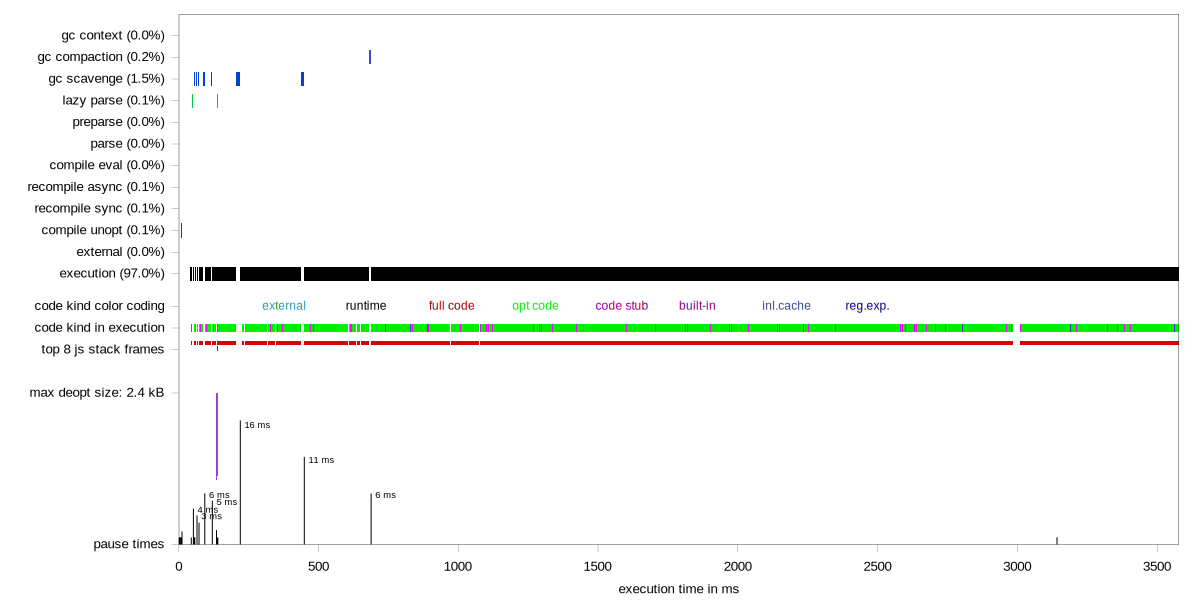
\includegraphics[width=16cm]{particles/particles2-profile.png}
\end{figure} 

The situation has also improved in the garbage collection log.

\lstinputlisting[caption=Garbage collection in optimised particle system,label=listing:particles2gc]{particles/particles2gc.txt}

\chapter{Sphere collision}
\label{cha:spherecollision}

Spheres are the simplest of bounding shapes used in collision detection. This chapter presents tests for two versions of algorithms -- naive $O(N^2)$ approach and with partitioned space. While the simpler algorithm has a far greater number of collision checks per frame, it allocates almost no memory per frame. A more complex method will minimise the number of checks, but additional structure and steps added may influence overall execution time in an unexpected way.


\begin{figure}[h!]
  \caption{Example rendering of tested sphere collision system}
  \label{img:spheres}
  \centering
	\includegraphics[width=16cm]{spheres/render.png}
\end{figure}

\section{Algorithm description}
\label{sec:spherealgorithmdescription}

Collision detection for spheres is a trivial task. If distance between two spheres is smaller than the sum of their radiuses, spheres collide.

$\sqrt{(S_1.x - S_2.x)^2 + (S_1.y - S_2.y)^2 + (S_1.z - S_2.z)^2} < S_1.radius + S_2.radius$

While the equation is simple, with the large number N of colliding objects the complexity of this detection is $O(N^2)$. Methods of space partitioning are used to reduce the number of checks. The one used in this benchmark is Octree.
The base for the algorithm is a tree-like structure of bounding boxes. Whenever a box contains more than one colliding object, it is divided into eight smaller boxes, by partitioning each edge by 2. When a maximum tree depth is reached, multiple objects are stored in one box. One object may be referenced from multiple boxes, when its size and position make them intersect. Each movement requires a check if the object has already moved to one of the neighbour boxes.

\begin{figure}[h!]
  \caption{Octree structure. Source: http://en.wikipedia.org/wiki/File:Octree2.svg/}
  \label{img:octree2}
  \centering
	\includegraphics[width=10cm]{octree/octree2.png}
\end{figure} 

Having objects grouped in boxes reduces the complexity of the collision check. Since an object may collide only with objects in the same box, the number of checks is much smaller. Overall complexity of Octree checks is $O(N log{N})$.

\begin{figure}[h!]
  \caption{Example of WebGL Octree debug rendering. Available online at http://pawlowski.it/octtree/}
  \label{img:octree}
  \centering
	\includegraphics[width=10cm]{octree/octree.png}
\end{figure} 

When collision is detected, collision response is calculated. From the rule of conservation of momentum:

\begin{center}
$m_1 * \vec{v_1} + m_2 * \vec{v_2} = m_1 * \vec{v'_1} + m_2 * \vec{v'_2}$
\end{center}

Meaning that change of both momentums is of equal value.
\begin{center}
$m_1*\vec{v'_1} =  m_1*\vec{v_1} - \Delta P$

$m_2*\vec{v'_2} =  m_2*\vec{v_2} + \Delta P$

$\vec{v'_1} =  \vec{v_1} - \frac{\Delta P}{m_1}$

$\vec{v'_2} =  \vec{v_2} + \frac{\Delta P}{m_2}$
\end{center}

To simplify response, rotation and deformation of spheres are ignored. This does not affect performance analysis, since operations in tests are performed all in the same way.

Let
\begin{center}
$P = |\Delta P|$

$N = \hat{pos_1 - pos_2}$
\end{center}

Since transference of momentum occurs only along single points of contact:
\begin{center}
$ \Delta P = P * \hat{\vec{N}}$

$\vec{v'_1} =  \vec{v_1} - \frac{P}{m_1} * \vec{N}$

$\vec{v'_2} =  \vec{v_2} + \frac{P}{m_2} * \vec{N}$
\end{center}

Let us split each velocity into two scalars, the perpendicular and parallel value of velocity vector, and introduce $\vec{Q}$, similar to $\vec{N}$, a perpendicular normalised vector lining along the exchanged momentum.

 \begin{center}
$\vec{v_1} =  a_1 * \vec{N} + b_1 * \vec{Q}$

$\vec{v_2} =  a_2 * \vec{N} + b_2 * \vec{Q}$

$\vec{v'_1} =  a'_1 * \vec{N} + b'_1 * \vec{Q}$

$\vec{v'_2} =  a'_2 * \vec{N} + b'_2 * \vec{Q}$
\end{center}

\begin{figure}[h!]
  \caption{Illustration for collision response}
  \label{img:spheresbounce}
  \centering
	\includegraphics[width=8cm]{spheres/bounce.jpg}
\end{figure} 

Deriving from previous equations:

 \begin{center}
$a_1' =  a_1 - \frac{P}{m_1}$

$b_1' = b_1$

$a_2' =  a_2 + \frac{P}{m_2}$

$b_2' = b_2$
\end{center}

Now let us use the rule of energy conservation to solve P:

 \begin{center}
$\frac{m_1}{2} * ||\vec{v_1}||^2 + \frac{m_2}{2} * ||\vec{v_2}||^2 = \frac{m_1}{2} * ||\vec{v'_1}||^2 + \frac{m_2}{2} * ||\vec{v'_2}||^2$

$\frac{m_1}{2} * ({a_1}^2 + {b_1}^2) + \frac{m_2}{2} * ({a_2}^2 + {b_2}^2) = \frac{m_1}{2} * ({a'_1}^2 + {b'_1}^2) + \frac{m_2}{2} * ({a'_2}^2 + {b'_2}^2)2$

$P = \frac{2*m_1*m_2*(a_1-a_2)}{m_1+m_2}$
\end{center}

and finally, using the result from the conservation of momentum:

 \begin{center}
$\vec{v'_1} =  \vec{v_1} - \frac{2*(a_1-a_2)}{m_1+m_2} * m_2 * \vec{N}$

$\vec{v'_2} =  \vec{v_2} + \frac{2*(a_1-a_2)}{m_1+m_2} * m_1 * \vec{N}$
\end{center}

From this result, using only the dot product of velocity vectors and normalised vector $pos_1 - pos_2$ the correct response to collision is calculated. In tested scenarios, the mass of all spheres is equal since it does not affect the complexity of calculations and produces less random results.


\section{{$O(N^2)$} approach}
\label{sec:sphereinitial}

The naive approach for collision detection proves to by easy to implement in JavaScript. Since almost no memory is allocated in each frame, no garbage collection issues appear. All methods are well defined and work mostly on floats. This results in a highly optimised binary code produced by the compiler, as shown on \ref{img:spheres1profile}.

\begin{figure}[h!]
  \caption{Chart of time used in optimised version of JavaScript}
  \label{img:spheres1profile}
  \centering
	\includegraphics[width=16cm]{spheres/spheres1-profile.png}
\end{figure} 

Multiple tests with N=1000 and different number of frames rendered show that for simple mathematical tasks, the performance of JavaScript is very close to that of C++. On average, the JavaScript version of benchmark runs 15\% longer than a C++ one.

\begin{figure}[h!]
  \caption{Comparison of total execution time. N = 1000, varying number of frames.}
  \label{img:spheres1-time-total}
  \centering
	\includegraphics[width=16cm]{spheres/time-total.png}
\end{figure} 
\begin{figure}[h!]
  \caption{Comparison of execution time per frame. N = 1000, varying number of frames.}
  \label{img:spheres1-time-per-frame}
  \centering
	\includegraphics[width=16cm]{spheres/time-per-frame.png}
\end{figure}

\section{Octree-partitioned space}
\label{sec:sphereoctree}

\begin{figure}[h!]
  \caption{Octree partitioned sphere collision system}
  \label{img:spheres}
  \centering
	\includegraphics[width=16cm]{spheres/render2.png}
\end{figure}

Tests with Octree partitioning were executed with N=1000 spheres and T=1000 frames. The varying value is the maximum depth of Octree, ranging from 1 to 10.
Changing the maximum depth reduces the number of collision checks between spheres, as shown on \ref{img:octree-collisions}.

\begin{figure}[h!]
  \caption{Number of collisions in Octree}
  \label{img:octree-collisions}
  \centering
	\includegraphics[width=16cm]{spheres/octree-collisions.png}
\end{figure}

For low values, the overall complexity of checks does not change significantly, since most spheres are in one or a few bounding cubes, and no checks are skipped. Additional operations related to Octree actually make this solution slower than $O(n^2)$ approach. For depth values in the optimal zone, the number of collisions is reduced by a factor of at least 10, while keeping Octree overhead reasonable. Interesting thing happens when the maximum level of Octree is very high and the edge of the smallest Octree cube approaches the size of the spheres. The number of transitions between partitioning cubes, related memory allocation and cleanups actually make this approach much slower, as shown on \ref{img:octree-time}. Moreover, some spheres are references in more than one cube, raising again the number of collision checks.

\begin{figure}[h!]
  \caption{Run times in Octree system}
  \label{img:octree-time}
  \centering
	\includegraphics[width=16cm]{spheres/octree-time.png}
\end{figure}

It's clearly visible that the number of collision checks and run time is correlated only up to a certain point. For deep Octrees, the number of checks does not improve further, but the overall run time gets longer. The performance of JavaScript in relation to C++ varies between 30\% to 80\% overhead. In comparison with $O(n^2)$ approach, optimal Octree in JavaScript runs over 92\% faster and C++ over 94\% faster.

\chapter{Emscripten}
\label{cha:emscripten}

JavaScript is often called an assembly language of the Web.\cite{javascript-assembly-of-web} One could argue that since only one language is supported by browsers it could be made a compilation target similar to an assembler for CPU. This statement is flawed, since eventually JavaScript is translated to assembly making it only an intermediate step. Probably, a resemblance to ByteCode in JVM, which is a compilation target of multiple languages like Java, Scala and Clojure is more in place.
Nevertheless, recent years have shown multiple projects aimed at converting code to JavaScript. Some introduce new syntax like CoffeeScript, Dart or TypeScript, while still serving the same purpose -- providing human readable code that is interpreted in browser on the fly. Others, which are the focus of this chapter, aim to convert existing projects to run in a browser.

Several new projects are connected to make this happen. The first steps in conversion between languages were made with the LLVM project\cite{llvm} which currently is a collection of tools and compilers converting code to and from intermediate representation (LLVM IR). For C++ Clang\cite{clang} is a conversion tool.

\begin{figure}[h!]
  \caption{Pipeline of Emscripten conversion. Source: \cite{javascript-assembly-of-web}}
  \label{img:emscriptenpipeline}
  \centering
	\includegraphics[width=8cm]{emscripten/pipeline.jpg}
\end{figure}

The code in LLVM is suitable for further conversion to language like JavaScript. This part is handled by the Emscripten\cite{emscripten} project. Initially, the compilation target for Emscripten was plain JavaScript. With recent developments the asm.js\cite{asmjs} library was created. It provides syntax built on top of JavaScript, which is strongly typed and easily translatable to assembly language. Asm.js details are explained in section \ref{sec:asmjsoverview}.

\lstinputlisting[caption=Example of code using asm.js,label=listing:asmjs]{emscripten/asm.js}

The project, built in cooperation with Mozilla Foundation, has its own engine for Firefox -- OdinMonkey, designed to run faster for this limited and well-defined syntax.

Altogether these projects resulted in multiple libraries and games converted from the native version to JavaScript.

Proof-of-concept demo, made in cooperation between Mozilla and Unreal, is Epic Citadel HTML5 -- Unreal Engine 3 technology demo\cite{epiccitadel}  instance running in the browser.\cite{epiccitadelhtml5} The companies claim it took only four days to complete the conversion.

\begin{figure}[h!]
  \caption{Epic Citadel screenshot}
  \label{img:epicitadel}
  \centering
	\includegraphics[width=16cm]{emscripten/epic-citadel.jpg}
\end{figure}

Another example of a successfully converted project is ammo.js\cite{ammojs} -- originating from the Bullet physics engine.

\begin{figure}[h!]
  \caption{Ammo.js demo colliding 500 boxes at 30fps, available at http://kripken.github.io/ammo.js/examples/new/ammo.html}
  \label{img:epicitadel}
  \centering
	\includegraphics[width=16cm]{emscripten/ammojs.png}
\end{figure}

\section{Asm.js overview}
\label{sec:asmjsoverview}

Asm.js introduces some improvements targeted to fix performance problems of JavaScript. Ahead of time compilation enforces very specific rules on the coding style. Documentation\cite{asmjs} lists:

\subsection{Unboxed representations of integers and floating-point numbers}
\label{sec:asmjsunboxed}
In asm.js the only types allowed are integers and doubles. All numbers have annotations indicating static type (see: \ref{listing:typestree}). This way, the compiler does not have to detect possible transitions between variable types, and the overall code runs faster.

\subsection{Absence of runtime type checks}
\label{sec:asmjstypechecks}
Since asm.js works only on well-defined numbers, all function calls are monomorphic and stable. In OdinMonkey ahead-of-time compilation is able to compile them to the most optimised version without tracking method calls. In engines using JIT, methods are compiled early and newer deoptimised.

\subsection{Absence of garbage collection}
\label{sec:asmjsgc}
As shown in previous chapters, garbage collection calls are often a performance bottleneck. Asm.js solves this problem by eliminating garbage collection completely. Memory is stored in short-life variables, deallocated after the method exits and in global heaps, which are never resized or deallocated.

\subsection{Efficient heap loads and stores}
\label{sec:asmjsheap}

Heaps are global arrays of statically typed arrays, in JavaScript implemented as objects listed in \ref{table:jsarrays}. The size of the heap does not change during runtime -- it has to be calculated during the compilation and incorrect prediction or memory leaks may result in buffer overflow. Heaps are always passed as an argument to asm.js modules. Each module may reference part of the heap and use it as long as necessary.

\begin{table}[h!]
\caption{Statically typed arrays in JavaScript}
\centering
\label{table:jsarrays}
\begin{tabular}{|l|l|l|}
  	\hline
View Type & Element Size (Bytes) & Element Type \\ \hline
Uint8Array & 1 & intish \\ \hline
Int8Array & 1 & intish \\ \hline
Uint16Array & 2 & intish \\ \hline
Int16Array & 2 & intish \\ \hline
Uint32Array & 4 & intish \\ \hline
Int32Array & 4 & intish \\ \hline
Float32Array & 4 & doublish \\ \hline
Float64Array & 8 & doublish \\ \hline
\end{tabular}
\end{table}

\subsection{Summary}
\label{sec:asmjssummary}

These solutions remove some of the performance bottlenecks described in previous chapters. The code suitable to run with asm.js is almost unreadable by the programmer, and resembles an assembly code. Asm.js is not designed to be a language used by a programmer, it is mainly a target for compilation using converters like Emscripten.

Most optimisation used by asm.js is consistent with the code that is expected by V8 engine -- variables and methods are monomorphic, garbage collection is close to zero. It is worth noting that a code written by hand is almost always shorter than one generated by Emscripten. A partial solution to this is the built-in Google Closure Compiler, used on output of Emscripten and different levels of optimisation.
In tests mentioned in this paper, all solutions take 2 to 4kB compiled, while Emscripten produces over 450kB of code for each. This affects real life performance by lengthening at least transfer and parse time for code. The average parse time of 1kB of JS is believed to be up to 1ms\cite{best-practices-mobile}. The global average bandwidth was 3.1 Mbps in Q1 2013\cite{stateoftheinternet} thus transfer of each kilobyte is around 2.5ms. In total, the load time of the tested code is approximately 1.5 second on an average bandwidth and platform. In the case of larger applications and games, the load time may be significantly greater and should be taken into consideration.

\chapter{Summary}
\label{cha:summary}

All four tests were compiled and run times were measured on different platforms. Results obtained from Windows platform are significantly better than on Linux or Mac OS X. Reason for this is probably process of compilation of V8 itself, which by design is a 32-bit program. All tested operating systems are 64-bit. Results on Windows will be used as a baseline, since it is a platform most often used for gaming. It is expected that performance on all platforms will become similar once V8 switches to 64-bit.

The unoptimised version of the particle system (see: \ref{sec:particlesinitial}) was designed to perform a lot of memory operations. In the tests it is visible that C++ handles this task best. The code generated using Emscripten benefits from static memory heap, which effectively works similar to the object pool introduced later, and runs approximately twice as long as C++. Plain JavaScript suffers greatly from memory allocation issues and an unoptimised code, resulting in 6 times slower execution than C++.

Optimised particles (see: \ref{sec:particlesobjectpool}) with an object pool and low garbage collection show how improvements of the algorithm result in much faster JavaScript execution. It still takes twice as long to run the particle system in V8, but the Emscripten version takes three times longer than C++. The additional overhead of a long and complex code is clearly visible, and since JS code employs the same techniques that Emscripten uses automatically, there is no improvement in the related areas. It is worth mentioning that the unoptimised version of C++ particle system is slightly slower than an optimised JavaScript one, showing that code quality improvement that does not affect algorithmic complexity of an algorithm may be more important than the choice of the environment.

\begin{table}[h!]
\caption{Particle tests on different platforms}
\label{table:benchmarks}
\begin{tabular}{|p{4cm}||l|l|l||l|l|l|}
  	\hline
   Platform & \multicolumn{3}{c}{Unoptimised particles} & \multicolumn{3}{c}{Optimised particles}\\ \hline
   & C++ & JavaScript & Emscripten & C++ & JavaScript & Emscripten\\ \hline
   Fedora 19, Intel i7 2670QM, 4GB RAM, g++ 4.8.1 & 3.21s & 19.51s & 4.85s & 1.63s & 4.96s & 5.10s \\ \hline
   Windows 7, Intel i7 2670QM, 4GB RAM, g++ 4.7.3, Cygwin & 3.51s & 20.77s & 6.46s & 1.71s & 3.47s & 5.57s \\ \hline
   Mac OS X 10.8.5, Intel i7 3720QM, 8GB RAM, XCode 5.0 & 1.83s & 16.91s & 4.16s & 1.22s & 2.35s & 4.23s \\hline
\end{tabular}
\end{table}

The sphere collision test is putting a high load on CPU.

In $O(n^2)$ version (see: \ref{sec:sphereinitial}) exactly 1 000 000 000 checks for object collisions are made. The overall execution time is surprisingly good for JavaScript with an overhead of approximately 15\% and for the Emscripten generated version -- 25\%. This is a result of focusing on pure mathematical operations that are quickly compiled by V8 and processed on unboxed numbers in asm.js.

Space partitioning using Octree greatly reduces the number of collisions (to less than 100 000) and execution time. To give meaningful results simulation time is increased from 1000 frames to 10000. Under these circumstances difference in run time changes to 20\% for Javascript and remains similarly around 25\% for Emscripten. This is the result of small memory operations related to Octree areas.

\begin{table}[h!]
\caption{Spheres tests on different platforms}
\label{table:benchmarks}
\begin{tabular}{|p{4cm}||l|l|l||l|l|l|}
   \hline
   Platform & \multicolumn{3}{c}{$O(n^2)$ spheres} & \multicolumn{3}{c}{Octree spheres}\\ \hline
   & C++ & JavaScript & Emscripten & C++ & JavaScript & Emscripten\\ \hline
   Fedora 19, Intel i7 2670QM, 4GB RAM, g++ 4.8.1 & 4.96s & 9.02s & 12.35s & 
3.44s & 14.14s & 11.20s \\ \hline
   Windows 7, Intel i7 2670QM, 4GB RAM, g++ 4.7.3, Cygwin & 9.52s & 10.81s & 11.82s & 14.10s & 16.95s & 17.79s \\\hline
   Mac OS X 10.8.5, Intel i7 3720QM, 8GB RAM, XCode 5.0 & 5.05s & 8.62s & 13.88s & 6.67s & 14.34s & 17.23s \\hline
\end{tabular}
\end{table}

The above results show how well-written JavaScript or properly converted C++ are able to perform in a browser with similar performance to native programs, rarely exceeding 100\% overhead and sometimes getting as close as 15\% to C++ execution time.

Conducted experiments show a gap between JavaScript and C++ performance. Significant language design differences result in code that is often easier to write, but also easier to abuse. Benchmarks show differences between 15\% and 100\% overhead for correctly designed JavaScript code and over 500\% for incorrect patterns. Considering Moore's law, stating that computers double speed every 18 months, it safe to say that JavaScript is very close to being suitable for any type of development.

Tests show a clear pattern regarding dynamic variable types in JavaScript. Whenever boxing and unboxing happens, JIT compilation is not able to properly optimise code and bring it up to the performance of C++. This affects both simple variables and properties and is especially visible for numbers. Transitions between integer and floats are expensive, while easy to overlook.

Types also significantly affect the cost of method calls. Keeping methods monomorphic in core parts of the physics engine is very important. An additional cost of polymorphism of parameters is not only boxing and unboxing of parameters, but also time spent on optimising and deoptimising the compiled method, which makes initial warmup of the engine longer. Exporting well defined methods to be called from polymorphic ones is an easy workaround for this performance bottleneck.

Lastly, memory management proven to be one of the most important problems in JavaScript. Automated garbage collection connected with the popular pattern of creating and returning arrays is an important problem. Memory allocation of objects is also a bottleneck, but not very dissimilar to the one in C++. As shown in the second version of the particle system, the usage of object pools and changing architecture to avoid array creation are techniques that can be employed to fight it. It is worth mentioning that while garbage collection always introduces some overhead, it is reasonable to avoid it at all costs. The sphere collision system with octree partitioning is also introducing and destroying objects, but overhead is significantly smaller than gained speedup. Advice for memory operations is to avoid objects living only for a single frame i.e. temporary variables and helpers. Long-living objects are in general unavoidable and should be used whenever suitable.

General advice for programming in JavaScript is to use techniques similar to those found in asm.js -- keep types static, method calls monomorphic and work carefully with memory.

Conducted tests show that while a gap between JavaScript and the native application exists and is not insignificant, there is a lot of potential in such an approach. It is expected, that with the growing community and interest from the game industry, new games will be released on browser within a few years. Performance issues may prevent works on AAA titles, but companies focused more on the social aspect of games and new trends in monetisation may create games targeted for different users. With capabilities of browsers equal to having an 18-month older machine, less graphically demanding titles like The Sims or World or Warcraft may certainly be ported to run in JavaScript.

\appendix
\include{rozdzialA}
\chapter{Source code}
\label{cha:sourcecode}


\section{Math utilities}
\label{sec:mathsource}

\lstinputlisting[caption=Math utilities in JavaScript,label=listing:mathjs,language=JavaScript]{math.js}
\lstinputlisting[caption=Math utilities in C++,label=listing:mathjs,language=C++]{math.cpp}

\section{Particle system}
\label{sec:particlesource}

\lstinputlisting[caption=Particle object in JavaScript,label=listing:particlejs,language=JavaScript]{particles/particle.js}
\lstinputlisting[caption=Particle object in C++,label=listing:particlejs,language=C++]{particles/particle.cpp}
\lstinputlisting[caption=Particle emitter object in JavaScript,label=listing:particleemitterjs,language=JavaScript]{particles/particleEmitter.js}
\lstinputlisting[caption=Particle emitter object in C++,label=listing:particleemittercpp,language=C++]{particles/particleEmitter.cpp}
\lstinputlisting[caption=Initial particle system object in JavaScript,label=listing:particlesystem1js,language=JavaScript]{particles/particleSystem.js}
\lstinputlisting[caption=Initial particle system in C++,label=listing:particlesystem1cpp,language=C++]{particles/particleSystem.cpp}
\lstinputlisting[caption=Optimised particle system object in JavaScript,label=listing:particlesystem2js,language=JavaScript]{particles/particleSystem2.js}
\lstinputlisting[caption=Optimised particle system in C++,label=listing:particlesystem2cpp,language=C++]{particles/particleSystem2.cpp}


\section{Spheres collision detection}
\label{sec:spheressource}

\lstinputlisting[caption=Sphere object in JavaScript,label=listing:spherejs,language=JavaScript]{spheres/sphere.js}
\lstinputlisting[caption=Sphere object in C++,label=listing:spherejs,language=C++]{spheres/sphere.cpp}

\lstinputlisting[caption=Sphere system object in JavaScript,label=listing:spheresystemjs,language=JavaScript]{spheres/sphereSystem.js}
\lstinputlisting[caption=Sphere system in C++,label=listing:spheresystemcpp,language=C++]{spheres/sphereSystem.cpp}


\lstinputlisting[caption=Octree in JavaScript,label=listing:octreejs,language=JavaScript]{spheres/octree.js}
\lstinputlisting[caption=Octree in C++,label=listing:octreecpp,language=C++]{spheres/octree.cpp}


\lstinputlisting[caption=Octree-based sphere system object in JavaScript,label=listing:spheresystem2js,language=JavaScript]{spheres/sphereSystem2.js}
\lstinputlisting[caption=Octree-based sphere system in C++,label=listing:spheresystem2cpp,language=C++]{spheres/sphereSystem2.cpp}


\clearpage
\phantomsection
\addcontentsline{toc}{chapter}{References}
\nocite{*}
\bibliographystyle{ieeetr}
\bibliography{bibliografia}

\end{document}
 
